\documentclass[12pt,a4paper]{ctexart}
\usepackage[margin=2.2cm]{geometry}
\usepackage{graphicx}
\usepackage{booktabs}
\usepackage{amsmath}
\usepackage{float}
\usepackage{hyperref}
\usepackage{xcolor}
\usepackage{listings}

\lstset{
	language=C,
	basicstyle=\ttfamily\small,
	keywordstyle=\color{blue!70!black},
	commentstyle=\color{green!40!black},
	stringstyle=\color{orange!60!black},
	showstringspaces=false,
	breaklines=true,
	frame=single,
	tabsize=2
}

\newcommand{\reporttitle}{实验二：类 C 语言词法分析器（Scanner）实现}
\newcommand{\subtask}{DFA 设计与词法记号输出}
\newcommand{\authname}{姓名}
\newcommand{\authid}{学号}

\title{\reporttitle}
\author{\authname：\underline{\hspace{3cm}} \quad \authid：\underline{\hspace{3cm}}}
\date{\today}

\begin{document}
\maketitle

\section{实验目的}
本实验围绕“类 C 语言词法分析器”展开，目标如下：
\begin{itemize}
	\item 根据给定词法规则，构建可执行的 DFA 思路并实现扫描器程序。
	\item 将源程序字符流切分为 token 序列，识别关键字、标识符、常数、运算符与界符。
	\item 将词法分析结果同时输出到终端与文件，作为后续语法分析阶段输入。
\end{itemize}

\section{实验过程}
\subsection{实验环境}
\begin{itemize}
	\item 操作系统：macOS
	\item 编程语言：C（C11）
	\item 编译工具：GCC
	\item 其他工具：LaTeX（ctexart）
\end{itemize}

\subsection{词法规则与输入形式}
本实验依据实验说明中的类 C 语言词法记号集合进行实现。核心规则如下：
\begin{itemize}
	\item 标识符：以字母或下划线开头，后续可接字母、数字、下划线。
	\item 整数与实数：支持无符号/带符号形式，其中实数支持小数点形式。
	\item 关键字：\texttt{int}、\texttt{float}、\texttt{void}、\texttt{if}、\texttt{else}、\texttt{while}、\texttt{return}、\texttt{input}、\texttt{print}。
	\item 关系运算符与赋值：\texttt{<, <=, >, >=, ==, !=, =}。
	\item 界符：\texttt{( ) [ ] \{ \} , ;}。
\end{itemize}

\subsection{实现步骤}
\begin{enumerate}
	\item 设计扫描器状态推进逻辑，维护当前字符、行列位置与前一 token 类型。
	\item 实现空白符与注释跳过（\texttt{//} 单行注释、\texttt{/* */} 多行注释）。
	\item 实现识别函数：标识符/关键字识别、数字识别、运算符与界符识别。
	\item 统一输出格式为 \texttt{(TOKEN, lexeme)}，并将结果写入 \texttt{tokens.out}。
	\item 在测试文件上运行，检查 token 序列正确性及错误统计信息。
\end{enumerate}

\section{实验内容}
\subsection{任务一：DFA 风格扫描器实现}
本任务使用 C 语言实现一个顺序扫描器。核心思想是“读取当前字符并转移到对应识别分支”，每次成功识别一个最长 token 后输出。

其中，数字处理支持以下情况：
\begin{itemize}
	\item 整数：如 \texttt{10}、\texttt{-3}。
	\item 浮点数：如 \texttt{3.14}、\texttt{-0.5}、\texttt{.75}。
\end{itemize}

为支持一元正负号与二元加减号区分，程序根据前一 token 是否为“值 token”判断当前 \texttt{+/-} 是否可并入数字。

\subsection{任务二：token 输出与错误处理}
识别到合法 token 后，输出到标准输出与结果文件。非法字符输出词法错误信息（带行列号）并继续扫描，最终给出错误总数。

本实验输出格式为：
\begin{equation}
\texttt{(TOKEN\_NAME, lexeme)}
\end{equation}

例如：\texttt{(VOID, void)}、\texttt{(ID, qsort)}、\texttt{(ROP, <=)}。

\section{实验结果}
\subsection{扫描结果截图}
\begin{figure}[H]
\centering
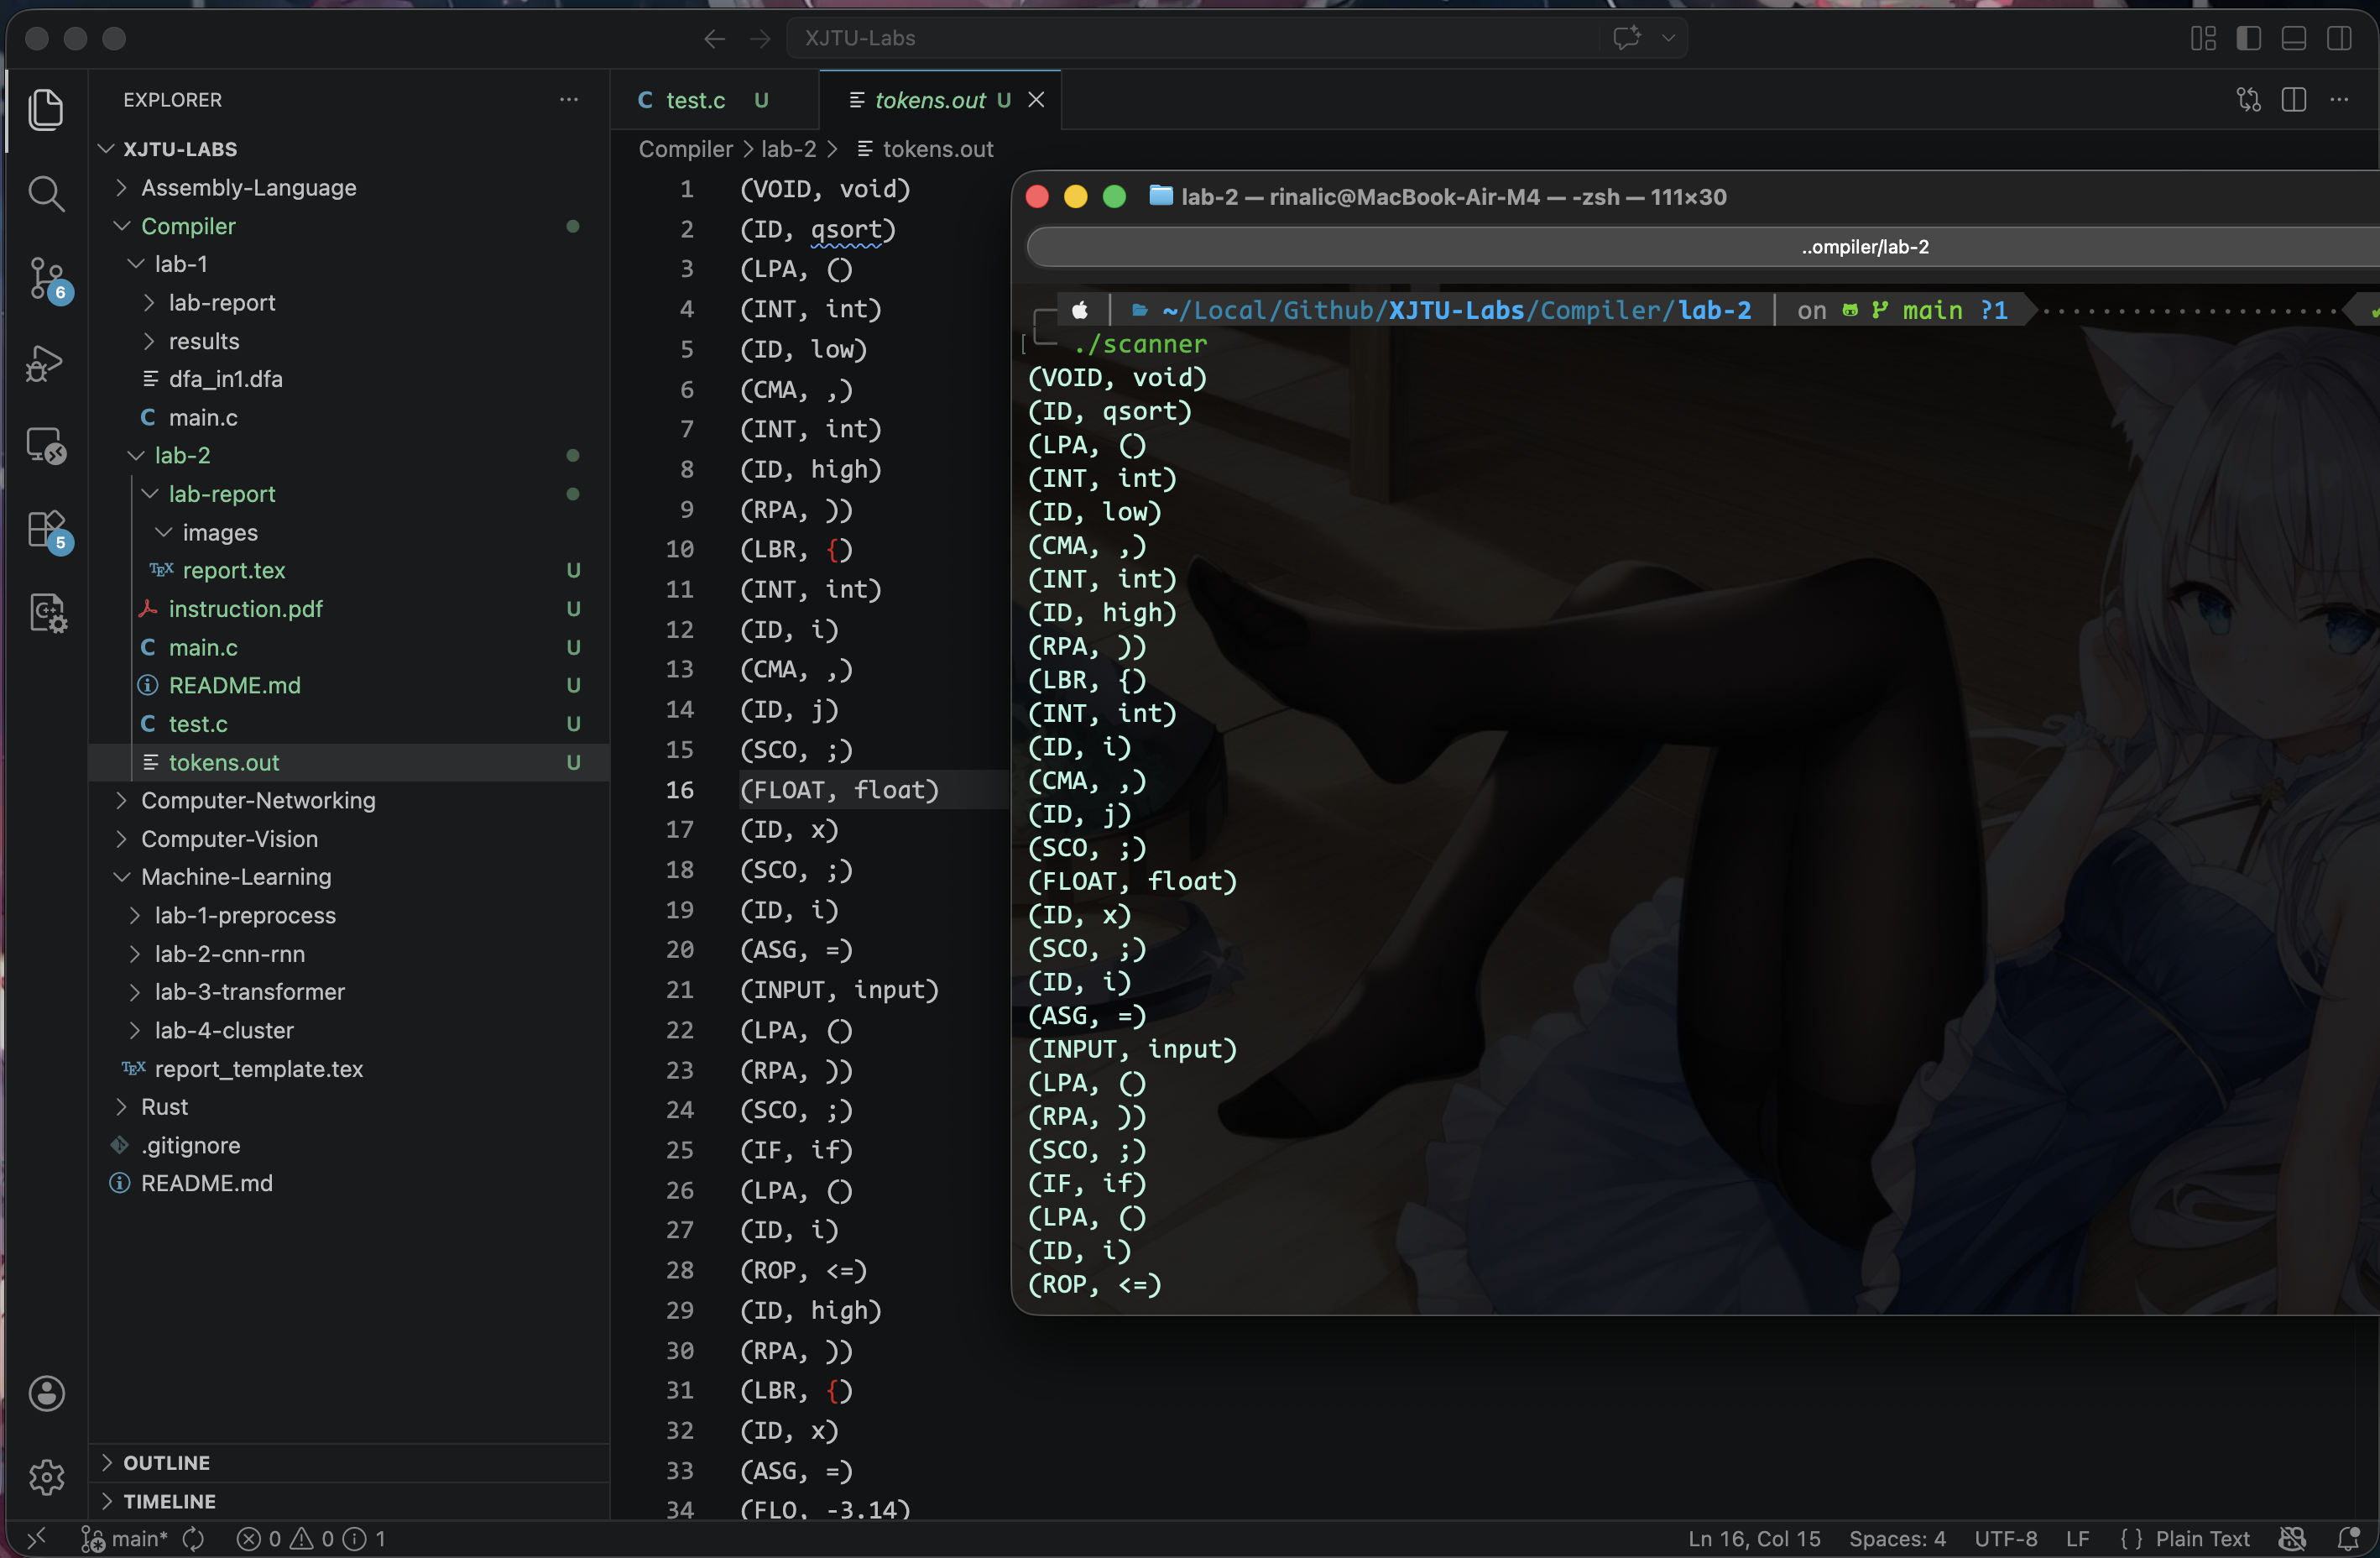
\includegraphics[width=0.95\textwidth]{images/run_result_default.png}
\caption{默认测试文件运行结果（终端 token 输出）}
\label{fig:run_result}
\end{figure}

结果分析：
\begin{itemize}
	\item 关键字、标识符、运算符、界符可被正确区分并按顺序输出。
	\item 浮点数 \texttt{-3.14} 被识别为 \texttt{FLO}，符合预期。
	\item 结果文件末尾显示 \texttt{Scanner finished with 0 lexical error(s).}，说明测试样例下扫描成功。
\end{itemize}

\subsection{代表性 token 统计}
\begin{table}[H]
\centering
\caption{样例程序中部分 token 统计}
\label{tab:token_count}
\begin{tabular}{lcc}
\toprule
token 类型 & 出现次数 & 示例 \\
\midrule
ID & 11 & \texttt{qsort, i, high} \\
INT & 4 & \texttt{int, 10, 1} \\
FLO & 1 & \texttt{-3.14} \\
ROP & 2 & \texttt{<=, <} \\
结构界符 & 15 & \texttt{( ) \{ \} ; ,} \\
\bottomrule
\end{tabular}
\end{table}

分析：该统计反映了样例程序包含函数定义、分支与循环结构，能够覆盖多数基础词法类型。

\section{总结}
本实验完成了类 C 语言 scanner 的设计与实现，达成了实验要求：
\begin{itemize}
	\item 基于 DFA 思路实现了可运行的词法分析器。
	\item 实现了关键 token 的识别与规范化输出。
	\item 实现了终端与文件双输出，可直接衔接后续语法分析阶段。
\end{itemize}

后续可改进方向：
\begin{itemize}
	\item 扩展字符串常量、字符常量等词法单元。
	\item 增加更细粒度错误恢复策略与错误分类。
	\item 将词法规则表格化，支持可配置词法定义。
\end{itemize}

\section*{附录：实验源代码}
\subsection*{A.1 主要源码：main.c}
\lstinputlisting{../main.c}

\subsection*{A.2 测试输入：test.c}
\lstinputlisting{../test.c}

\subsection*{A.3 运行命令}
\begin{verbatim}
# 在 Compiler/lab-2 目录下
gcc -std=c11 -Wall -Wextra -O2 main.c -o scanner

# 默认读取 test.c，输出到 tokens.out
./scanner

# 指定输入输出文件
./scanner test.c tokens.out
\end{verbatim}

\end{document}
